\chapter{Zahtevi za realizacijom sistema}\label{zahtevi}
\section{Korisnički zahtevi}
Korisnički zahtevi se mogu podeliti u dve grupe. To su:
\begin{enumerate}
\item Zahtevi platforme generalne namene za polaganje, ocenjivanje i administraciju testova
\item Zahtevi sistema za parsiranje, transformisanje i prikazivanje logičkih izraza
\end{enumerate}
\subsection{Prva grupa zahteva}
Prva grupa zahteva se odnosi na samu platformu za polaganje testova. \subsubsection{Logovanje i registracija}
Kako je sistem namenjen za upotrebu od strane studenata i administratora, neophodno je implementirati logovanje postojećih korisnika na sistem i registraciju novih korisnika. Pri tom je bitno razlikovati login standardnih korisnika i administratora. Osim toga što ove dve role koriste sistem na različit način, administrator ima neke privilegije koje nisu dostupne običnom korisniku - na primer, pregledanje rezultata testova. O ovome se mora voditi računa, tako da se onemogući pristup resursima za koje su potrebne administratorske privilegije.

Logovanje treba da se vrši preko studentskog email naloga i lozinke. Novi korisnici se registruju tako što unesu email adresu, na koju se potom šalje nasumično generisana lozinka. Lozinke se od klijenta ka serveru treba da se šalju u heširanom obliku, a u istom obliku treba da se pohranjuju u bazi podataka. Administratoski nalozi se automatski ubacuju u bazu prilikom konfiguracije sistema.

Nakon što se korisnik uloguje, preko kolačića u pregledaču treba da se pamti korisnička sesija, i time izbegava ponovno, nepotrebno logovanje na sistem nakon napuštanja stranice. Sesije treba da ima određeno vreme validnosti, nakon kojeg je neophodno da se korisnik ponovo uloguje.

Korisnik treba da ima izbor da se izloguje kada poželi, i time invalidira korisničku sesiju.

\subsubsection{Pregled testova}
Nakon uspešnog logovanja, korisnik treba da vidi spisak svih testova koje trenutno može da polaže, grupisanih po oblasti. Među ovim testovima treba da se nalaze i testovi koje je korisnik već polagao - oni trebaju biti onemogućeni, tj. korisniku ne sme biti dozvoljeno da više puta polaže isti test. Za testove koje su položeni treba da se naznači datum polaganja i uspešnost, tj. broj pitanja na koje je student tačno odgovorio u odnosu na ukupan broj pitanja na testu. Za testove koji su u toku, tj. čije je polaganje korisnik započeo, ali nije završio, treba naznačiti trenutni progres, odnosno broj pitanja na koja je student dao odgovor naspram ukupnog broja pitanja na testu.

\subsubsection{Polaganje testova}
Svaki test treba da se sastoji iz određenog broja pitanja, grupisanih po stranicama. Svaka stranica, uz pitanja, može opciono da sadrži i \textit{demonstraciju}, koja može biti slika, animacija, jednačina, interaktivni element itd. Postoje tri tipa pitanja:
\begin{itemize}
\item pitanja sa više ponuđenih, a jednim tačnim odgovorom - odgovarajuća komponenta je \textit{radio button},
\item pitanja sa više ponuđenih i više tačnih odgovora - odgovarajuća komponenta je \textit{checkbox}, i
\item pitanja sa odgovorom u slobodnom stilu - odgovarajuća komponenta je tekstualno polje.
\end{itemize}
Primer jedne stranice sa pitanjima dat je na slici \ref{fig-test}.
\begin{figure}[h]
\label{fig-test}
\centering
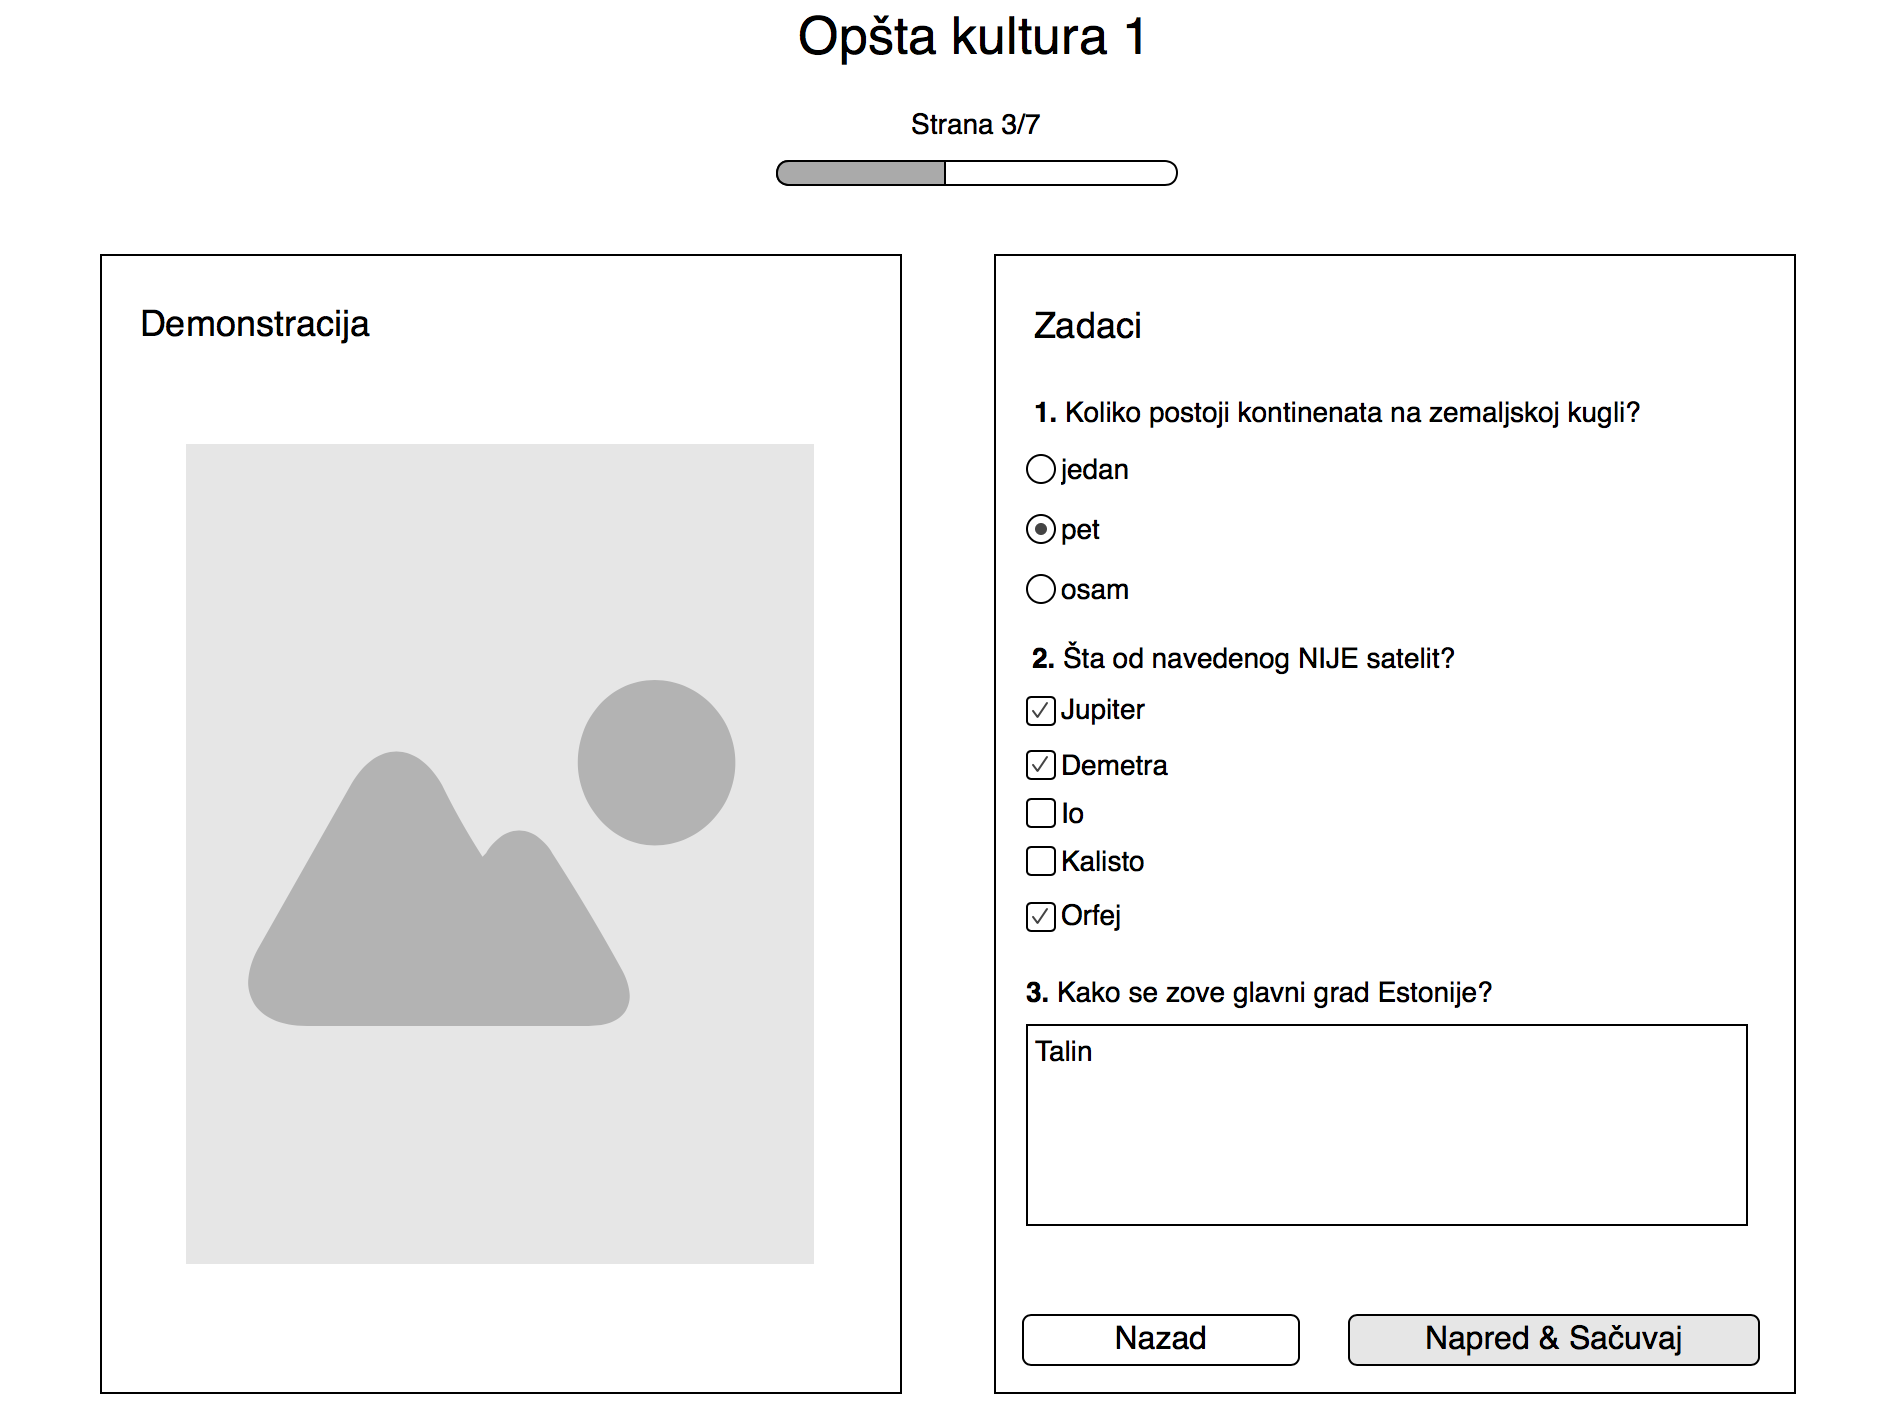
\includegraphics[width=\textwidth]{test-mockup}
\caption{UI \textit{mockup} stranice za polaganje testova}
\end{figure}

Korisnik može slobodno da se kreće kroz stranice sa pitanjima. Pri tome se čuvaju uneti odgovori na pitanja. Korisnik može preskočiti neka pitanja, ali mu se tada, pre predavanja testa, prikazuje upozorenje da na neka pitanja nije dat odgovor.

Nakon što korisnik odgovori na sva pitanja sa testa, na poslednjoj stranici treba da se pojavi dugme za predavanje testa. Kada korisnik klikne na ovo dugme, test treba da bude automatski ocenjen i trajno unet u bazu. Korisnika tada treba vratiti na stranicu za pregled testova. Time je proces polaganja testa završen.

Ukoliko korisnik u bilo kom trenutku prekine polaganje testa, potrebno je omogućiti nastavljanje polaganja prilikom sledećeg logovanja korisnika. Naravno, treba restaurirati dotadašnji progres polaganja testa.

\section{Opis korišćenih tehnologija}
\subsection{Izbor jezika}
Online platforma poput izrađene web aplikacije se može realizovati u gotovo svim višim programskim jezicima današnjice. Prednost svakako imaju jezici koji:
\begin{itemize}
\renewcommand\labelitemi{--}
\item su na dovoljno visokom nivou apstrakcije - na primer, podrška za \textit{garbage collection} je obavezna,
\item koji se mogu izvršavati na velikom broju platformi uz minimalne izmene izvornog koda - pre svega, interpreterski jezici i jezici koji se izvršavaju na virtuelnim mašinama, tj. prevode se u bajtkod,
\item dolaze sa kvalitetnom i robusnom standardnom bibliotekom, i za koje postoji veliki broj dostupnih \textit{3rd party} biblioteka, i
\item imaju detaljnu i preglednu dokumentaciju i podršku online zajednice.
\end{itemize}
Sa ovim ne pretarano striktnim ograničenjima na umu, prirodno se nameće veliki broj popularnih jezika: Java, C\#, Python, Go, Rust itd.

Međutim, kako autor tokom dužine studija nije imao priliku da izučava još neku paradigmu osim objektno-orijentisanog programiranja, a vođen idejom da jedan alat nikako ne može da bude pravo rešenje za sve probleme, odluka je pala na \textbf{Clojure}. Clojure je moderni dijalekat LISP-a, i samim tim je funkcionalan jezik. Izvorni kod Clojure programa se prevodi na Java bajtkod, koji se izvršava na Java virtuelnoj mašini\footnote{Osim Java bajtkoda, Clojure kod je moguće pokretati i na \textit{Common Language Runtime} mašini i JavaScript mašini.}. Zbog toga Clojure, pored već bogatog ekosistema raznoraznih biblioteka, ima pristup svim bibliotekama pisanim u Javi. Takođe, Clojure ima veoma aktivnu zajednicu, kao i veliki broj knjiga\cite{Emerick:2012:CP}\cite{Higginbotham:2015:CBT}, priručnika, tutorijala i resursa za učenje.

Jedna prednost Clojure-a nad Javom, koju će autor vremenom naučiti da veoma ceni, jeste postojanje \textbf{REPL} (\textit{read-eval-print-loop}) funkcionalnosti. Radi se o interaktivnoj konzoli u kojoj je moguće unositi i evaluirati delove Clojure koda, veoma slično Python interpreteru. Uz činjenicu da su većina Clojure funkcija \textit{pure}\footnote{Čiste funkcije uvek vraćaju isti rezultat za iste argumente, i nemaju bočne efekte.}, REPL omogućava unikatan način razvijanja aplikacije, gde je funkcija osnovna celina razvoja i testiranja.

Izrađena web aplikacija se sastoji od dva snažno spregnuta dela: \emph{frontend} sistema i \emph{backend} sistema. Kao što im ime kaže, frontend deo je zadužen za prezentacioni sloj i obradu unosa, dok je backend sistem zadužen za perzistenciju i serviranje sadržaja, i veći deo poslovne logike.

\subsection{Backend}

\paragraph{HTTP server}
\emph{Ring}\cite{ring} je apstrakcija HTTP servera koja preko veoma jednostavnog API-ja\footnote{\url{https://github.com/ring-clojure/ring/blob/master/SPEC}} omogućava korisniku da se fokusira na implementaciju hendlera (tj. poslovne logike), bez ulaženja u detalje HTTP protokola. API definiše HTTP zahtev i HTTP odgovor kao dve obične Clojure mape, a hendlere kao funkcije koje imaju jedan argument (mapu zahteva) i vraćaju odgovor kao mapu. Zbog toga što Ring predstavlja apstrakciju HTTP servera, Ring web aplikacije mogu da se distribuiraju kao WAR aplikacije i pokreću unutar standardnih kontejnera za web aplikacije (npr. Tomcat), ili da se pokrenu same pomoću \textit{embedded} Jetty web servera, što je za potrebe ove web aplikacije više nego dovoljno.

\paragraph{Rutiranje}
Ring API je previše jednostavan za neke iole ozbiljnije zahteve, te je zbog toga nastao \emph{Compojure}\cite{compojure}, koji je \textit{routing} biblioteka za Clojure. Jednostavno rečeno, ova biblioteka prosleđuje određene HTTP zahteve (\texttt{GET}, \texttt{POST} itd.) za URI putanjama (tj. resursima) hendlerima koji ih obrađuju. Tako je, na primer, moguće napraviti hendler koji vraća početnu stranicu ukoliko se ka serveru uputi HTTP \texttt{GET} zahtev za \texttt{/index.html} resursom. Međutim, \texttt{POST} zahtevi ka istom resursu će biti odbijeni sa statusom \texttt{403 Forbidden}. Ovaj postupak uparivanja resursa i hendlera se naziva rutiranje.

\paragraph{Perzistencija}
Kako korisnički zahtevi nameću, svi podaci o testovima, polaganju testova, registrovanim korisnicima itd. moraju se trajno negde smestiti, tj. moraju biti perzistentni. Standardna rešenja za perzistenciju predstavljaju relacione baze podataka. Autor se odlučio za \emph{PostgreSQL}\cite{postgres}, pre svega zbog postojećeg iskustva sa ovim RDBM sistemom.

\paragraph{Objektno-relaciono mapiranje}
ORM je strategija povezivanja stanja objekata u memoriji sa stanjem odgovarajućih objekata u relacionoj bazi. Iako su Clojure programima dostupne Java biblioteke koje predstavljaju industrijski standard (na primer, Hibernate), autor se odlučio za laganiju varijantu - za pristup bazi se koristi JDBC drajver za Postgres i mala Clojure biblioteka zvana \emph{YeSQL}\footnote{\url{https://github.com/krisajenkins/yesql}}. Ova biblioteka čita SQL skripte sa upitima, i za svaki upit pravi Clojure funkciju preko kojih je moguće proslediti imenovane parametre u upit, na sličan način na koji se to radi sa \texttt{NamedQuery} objektima u \textit{Java Persistence Language}-u. Nije razmatrana upotreba \textit{connection pooling}-a za konekcije ka bazi. Međutim, ukoliko se ukaže potreba za time, dodavanje takve biblioteke je prosto.

\paragraph{Logovanje} Za logovanje se koriste već dobro poznata rešenja u vidu \emph{Log4j} biblioteke i \emph{SLF4j} fasade. Konfiguracija se vrši putem tekstualnog fajla.

\subsection{Frontend}
